\begin{figure*}
    \centering
    \begin{subfigure}[b]{0.164\linewidth}
        \centering
        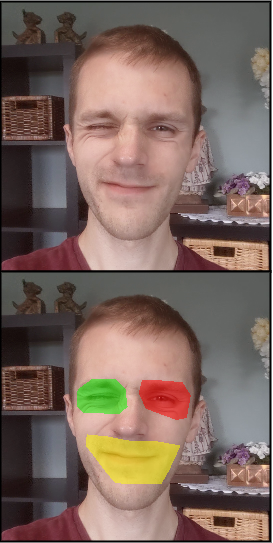
\includegraphics[width=\linewidth]{fig/assets/annotate/input.png}
        \caption{annotation}
    \end{subfigure}
    \hfill{}
    \begin{subfigure}[b]{0.816\linewidth}
        \centering
        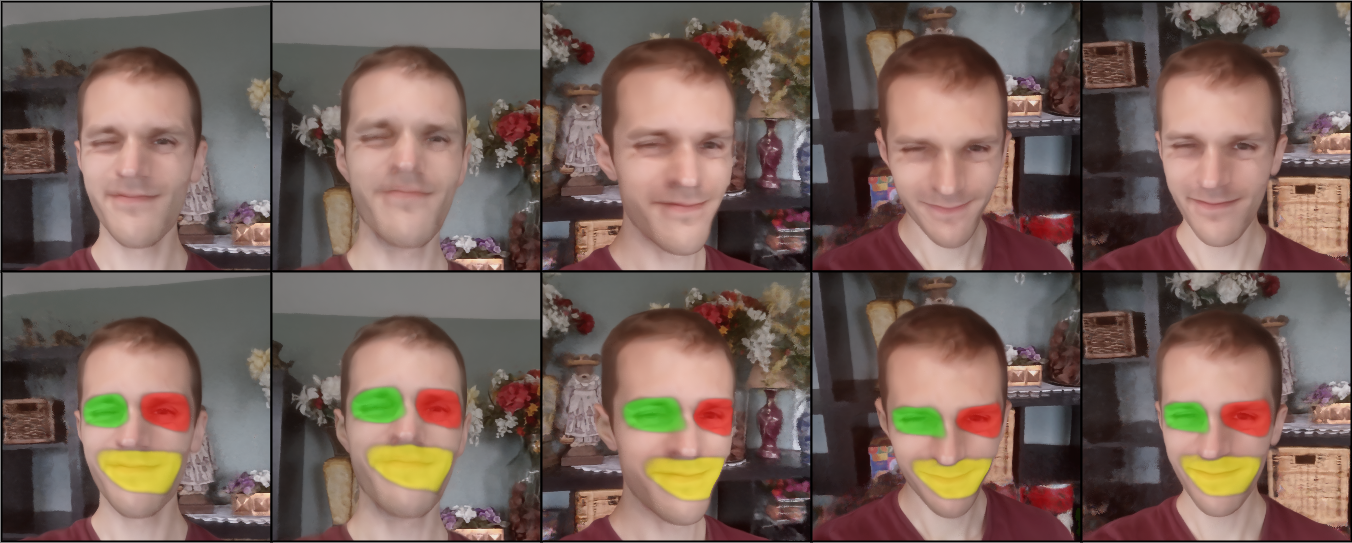
\includegraphics[width=\linewidth]{fig/assets/annotate/novel-views.png}
        \caption{unannotated views}
    \end{subfigure}
    \caption{{\bf Annotation example -- }
    We provide only a rough annotation for each attribute, which is enough for the method to discover the mask for each attribute across all views automatically.
    Bottom row shows masks overlaid on the image.
    }
    \label{fig:annotate}
\end{figure*}